% -----------------------------*- LaTeX -*------------------------------
\documentclass[UTF8]{report}
% ------------------------------------------------------------------------
% Packages
% ------------------------------------------------------------------------
\usepackage{adjustbox}
\usepackage{algorithm,algorithmicx}
\usepackage[noend]{algpseudocode}
\usepackage{amsmath,amsfonts,amssymb,bm,amsthm} % 数学宏包、数学字体、数学符号、支持 \mathscr{} 字体、支持粗斜体 \bm{}、数学定理
\usepackage{bigstrut,multirow,rotating} % Excel表格自动导入latex
\usepackage{booktabs}
\usepackage{breqn}
\usepackage{caption}
\usepackage{color} % 支持颜色改变
\usepackage{ctex}
\usepackage{enumitem} % 自定义列表环境
\usepackage{esint} % 支持多种积分算子
\usepackage{extarrows} % 任意长度的箭头
\usepackage{fancyhdr}
\usepackage{fontsize}
\usepackage{fontspec}
\usepackage[body={7in, 9in},left=1in,right=1in]{geometry}
\usepackage{graphicx} % 支持 \includegraphics{} 插图
\usepackage{mathrsfs}
\usepackage{mathtools} % 数学宏包的重要补充
\usepackage[framemethod=TikZ]{mdframed}
\usepackage{nicefrac}
\usepackage{scribe}
\usepackage{subfigure} % 插入子图
\usepackage{tikz,xcolor} % 画图、画 Feynman 图
\usepackage{upgreek} % 数学环境的直立希腊字母
\usepackage{colortbl} % 表格颜色
% ------------------------------------------------------------------------
% Macros
% ------------------------------------------------------------------------
%~~~~~~~~~~~~~~~
% Utility latin
%~~~~~~~~~~~~~~~
\newcommand{\ie}{\textit{i.e.}}
\newcommand{\eg}{\textit{e.g.}}
%~~~~~~~~~~~~~~~
% Environment shortcuts
%~~~~~~~~~~~~~~~
\newcommand{\balign}[1]{\ealign{\begin{align}#1\end{align}}}
\newcommand{\baligns}[1]{\ealigns{\begin{align*}#1\end{align*}}}
\newcommand{\bitemize}[1]{\eitemize{\begin{itemize}#1\end{itemize}}}
\newcommand{\benumerate}[1]{\eenumerate{\begin{enumerate}#1\end{enumerate}}}
%~~~~~~~~~~~~~~~
% Text with quads around it
%~~~~~~~~~~~~~~~
\newcommand{\qtext}[1]{\quad\text{#1}\quad}
%~~~~~~~~~~~~~~~
% Shorthand for math formatting
%~~~~~~~~~~~~~~~
\newcommand{\mbb}[1]{\mathbb{#1}}
\newcommand{\mbi}[1]{\boldsymbol{#1}} % Bold and italic (math bold italic)
\newcommand{\mbf}[1]{\mathbf{#1}}
\newcommand{\mc}[1]{\mathcal{#1}}
\newcommand{\mrm}[1]{\mathrm{#1}}
\newcommand{\tbf}[1]{\textbf{#1}}
\newcommand{\tsc}[1]{\textsc{#1}}
% \def\<{{\langle}}
% \def\>{{\rangle}}
\newcommand{\sT}{\sf T}
\newcommand{\grad}{\nabla}
\newcommand{\Proj}{\Pi}
%~~~~~~~~~~~~~~~
% Common sets 定义数集符号
%~~~~~~~~~~~~~~~
\newcommand{\R}{\mathbb{R}}
\newcommand{\Z}{\mathbb{Z}}
\newcommand{\Q}{\mathbb{Q}}
\newcommand{\N}{\mathbb{N}}
\newcommand{\C}{\mathbb{C}}
\newcommand{\reals}{\mathbb{R}} % Real number symbol
\newcommand{\integers}{\mathbb{Z}} % Integer symbol
\newcommand{\rationals}{\mathbb{Q}} % Rational numbers
\newcommand{\naturals}{\mathbb{N}} % Natural numbers
\newcommand{\complex}{\mathbb{C}} % Complex numbers
%~~~~~~~~~~~~~~~
% Common functions
%~~~~~~~~~~~~~~~
\renewcommand{\exp}[1]{\operatorname{exp}\left(#1\right)} % Exponential
\newcommand{\indic}[1]{\mbb{I}\left(#1\right)} % Indicator function
\newcommand{\indicsub}[2]{\mbb{I}_{#2}\left(#1\right)} % Indicator function
\newcommand{\argmax}{\mathop\mathrm{arg\, max}} % Defining math symbols
\newcommand{\argmin}{\mathop\mathrm{arg\, min}}
\renewcommand{\arccos}{\mathop\mathrm{arccos}}
\newcommand{\dom}{\mathop\mathrm{dom}} % Domain
\newcommand{\range}{\mathop\mathrm{range}} % Range
\newcommand{\diag}{\mathop\mathrm{diag}}
\newcommand{\tr}{\mathop\mathrm{tr}}
\newcommand{\abs}{\mathop\mathrm{abs}}
\newcommand{\card}{\mathop\mathrm{card}}
\newcommand{\sign}{\mathop\mathrm{sign}}
\newcommand{\prox}{\mathrm{prox}} % prox
\newcommand{\rank}[1]{\mathrm{rank}(#1)}
\newcommand{\supp}[1]{\mathrm{supp}(#1)}
\newcommand{\norm}[1]{\lVert#1\rVert}
%~~~~~~~~~~~~~~~
% Common probability symbols
%~~~~~~~~~~~~~~~
\newcommand{\family}{\mathcal{P}} % probability family / statistical model
\newcommand{\iid}{\stackrel{\mathrm{iid}}{\sim}}
\newcommand{\ind}{\stackrel{\mathrm{ind}}{\sim}}
\newcommand{\E}{\mathbb{E}} % Expectation symbol
\newcommand{\Earg}[1]{\E\left[#1\right]}
\newcommand{\Esubarg}[2]{\E_{#1}\left[#2\right]}
\renewcommand{\P}{\mathbb{P}} % Probability symbol
\newcommand{\Parg}[1]{\P\left(#1\right)}
\newcommand{\Psubarg}[2]{\P_{#1}\left[#2\right]}
% \newcommand{\Cov}{\mrm{Cov}} % Covariance symbol
% \newcommand{\Covarg}[1]{\Cov\left[#1\right]}
% \newcommand{\Covsubarg}[2]{\Cov_{#1}\left[#2\right]}
% \newcommand{\model}{\mathcal{P}} % probability family / statistical model
%~~~~~~~~~~~~~~~
% Distributions
%~~~~~~~~~~~~~~~
% \newcommand{\Gsn}{\mathcal{N}}
% \newcommand{\Ber}{\textnormal{Ber}}
% \newcommand{\Bin}{\textnormal{Bin}}
% \newcommand{\Unif}{\textnormal{Unif}}
% \newcommand{\Mult}{\textnormal{Mult}}
% \newcommand{\NegMult}{\textnormal{NegMult}}
% \newcommand{\Dir}{\textnormal{Dir}}
% \newcommand{\Bet}{\textnormal{Beta}}
% \newcommand{\Gam}{\textnormal{Gamma}}
% \newcommand{\Poi}{\textnormal{Poi}}
% \newcommand{\HypGeo}{\textnormal{HypGeo}}
% \newcommand{\GEM}{\textnormal{GEM}}
% \newcommand{\BP}{\textnormal{BP}}
% \newcommand{\DP}{\textnormal{DP}}
% \newcommand{\BeP}{\textnormal{BeP}}
% \newcommand{\Exp}{\textnormal{Exp}}
%~~~~~~~~~~~~~~~
% Theorem-like environments
%~~~~~~~~~~~~~~~
% \theoremstyle{definition}
% \newtheorem{definition}{Definition}
% \newtheorem{example}{Example}
% \newtheorem{problem}{Problem}
% \newtheorem{lemma}{Lemma}
%~~~~~~~~~~~~~~~
% 组合数学的模板和作业里用到的一些宏包和自定义命令
%~~~~~~~~~~~~~~~
\renewcommand{\emph}[1]{\begin{kaishu}#1\end{kaishu}}
\newcommand{\falfac}[1]{^{\underline{#1}}}
\newcommand{\binomfrac}[2]{\frac{#1^{\underline{#2}}}{#2!}}
\newcommand{\ceil}[1]{\left\lceil #1 \right\rceil}
\newcommand{\floor}[1]{\left\lfloor #1 \right\rfloor}
\newcommand{\suminfty}[2]{\sum_{#1=#2}^{\infty}}
\newcommand{\suminftyk}[0]{\sum_{k=0}^{\infty}}
\newcommand{\sumint}[3]{\sum_{#1=#2}^{#3}}
\newcommand{\sumintk}[2]{\sum_{k=#1}^{#2}}
\newcommand{\suminti}[2]{\sum_{i=#1}^{#2}}
%~~~~~~~~~~~~~~~
% 定义新命令
%~~~~~~~~~~~~~~~
\newcommand*{\unit}[1]{\mathop{}\!\mathrm{#1}}
\newcommand*{\dif}{\mathop{}\!\mathrm{d}}%微分算子 d
\newcommand*{\pdif}{\mathop{}\!\partial}%偏微分算子
\newcommand*{\cdif}{\mathop{}\!\nabla}%协变导数、nabla 算子
\newcommand*{\laplace}{\mathop{}\!\Delta}%laplace 算子
\newcommand*{\deriv}[2]{\frac{\mathrm{d} #1}{\mathrm{d} {#2}}}
\newcommand*{\derivh}[3]{\frac{\mathrm{d}^{#1} #2}{\mathrm{d} {#3^{#1}}}}
\newcommand*{\pderiv}[2]{\frac{\partial #1}{\partial {#2}}}
\newcommand*{\pderivh}[3]{\frac{\partial^{#1} #2}{\partial {#3^{#1}}}}
\newcommand*{\dderiv}[2]{\dfrac{\mathrm{d} #1}{\mathrm{d} {#2}}}
\newcommand*{\dderivh}[3]{\dfrac{\mathrm{d}^{#1} #2}{\mathrm{d} {#3^{#1}}}}
\newcommand*{\dpderiv}[2]{\dfrac{\partial #1}{\partial {#2}}}
\newcommand*{\dpderivh}[3]{\dfrac{\partial^{#1} #2}{\partial {#3^{#1}}}}
\newcommand{\me}[1]{\mathrm{e}^{#1}}%e 指数
\newcommand{\mi}{\mathrm{i}}%虚数单位
% \newcommand{\mc}{\mathrm{c}}%光速 定义与mathcal冲突
\newcommand{\red}[1]{\textcolor{red}{#1}}
\newcommand{\blue}[1]{\textcolor{blue}{#1}}
% \newcommand{\Rome}[1]{\setcounter{rome}{#1}\Roman{rome}}
%~~~~~~~~~~~~~~~
% 公式环境中箭头符号的简写
%~~~~~~~~~~~~~~~
\newcommand{\ra}{\rightarrow}
\newcommand{\Ra}{\Rightarrow}
\newcommand{\la}{\leftarrow}
\newcommand{\La}{\Leftarrow}
\newcommand{\lra}{\leftrightarrow}
\newcommand{\Lra}{\Leftrightarrow}
\newcommand{\lgla}{\longleftarrow}
\newcommand{\Lgla}{\Longleftarrow}
\newcommand{\lgra}{\longrightarrow}
\newcommand{\Lgra}{\Longrightarrow}
\newcommand{\lglra}{\longleftrightarrow}
\newcommand{\Lglra}{\Longleftrightarrow}
%~~~~~~~~~~~~~~~
% 一些数学的环境设置
%~~~~~~~~~~~~~~~
% \newcounter{counter_exm}\setcounter{counter_exm}{1}
% \newcounter{counter_prb}\setcounter{counter_prb}{1}
% \newcounter{counter_thm}\setcounter{counter_thm}{1}
% \newcounter{counter_lma}\setcounter{counter_lma}{1}
% \newcounter{counter_dft}\setcounter{counter_dft}{1}
% \newcounter{counter_clm}\setcounter{counter_clm}{1}
% \newcounter{counter_cly}\setcounter{counter_cly}{1}
% \newtheorem{theorem}{{\hskip 1.7em \bf 定理}}
% \newtheorem{lemma}[theorem]{\hskip 1.7em 引理}
% \newtheorem{proposition}[theorem]{Proposition}
% \newtheorem{claim}[theorem]{\hskip 1.7em 命题}
% \newtheorem{corollary}[theorem]{\hskip 1.7em 推论}
% \newtheorem{definition}[theorem]{\hskip 1.7em 定义}
\newcommand{\problem}[1]{{\setlength{\parskip}{10pt}\noindent \bf{#1}}}
\newenvironment{solution}{{\noindent\hskip 2em \bf 解 \quad}}{}
\renewenvironment{proof}{{\setlength{\parskip}{7pt}\noindent\hskip 2em \bf 证明 \quad}}{\hfill$\qed$\par}
% \newenvironment{example}{{\noindent\hskip 2em \bf 例 \arabic{counter_exm}\quad}}{\addtocounter{counter_exm}{1}\par}
% \newenvironment{concept}[1]{{\bf #1\quad} \begin{kaishu}} {\end{kaishu}\par}
%~~~~~~~~~~~~~~~
% 本.tex文档中特殊定义命令
%~~~~~~~~~~~~~~~
\newcommand{\cdclass}[2]{[#1]_{\text{#2}}}

% ----------------------------------------------------------------------
% Header information
% ------------------------------------------------------------------------

\begin{document}

\course{B0911006Y-01} 			%optional
\coursetitle{Computer Organization and Design}	%optional
\semester{2023 Spring}		%optional
\lecturer{Ke Zhang}	%optional
\scribe{吉骏雄}		%required
\lecturenumber{10}			%required (must be a number)
\lecturedate{June 5}	%required (omit year)

\maketitle

% ----------------------------------------------------------------------
% Body of the document
% ------------------------------------------------------------------------


\textbf{课后习题10.2, 10.7, 10.8, 10.15, 10.21}

\problem{10.2} 写出完成下列指令的微操作及节拍安排 (包括取指操作) . 
\begin{enumerate}[label=(\arabic*)]
    \item 指令 ``ADD $\mathrm{R_1}$, X'' 完成将$\mathrm{R_1}$寄存器的内容和主存X单元的内容相加结果存于$\mathrm{R_1}$的操作. 
    \item 指令 ``ISZ X'' 完成将主存X单元的内容增1, 并根据其结果若为0, 则跳过下一条指令执行. 
\end{enumerate}

\begin{solution}
    \begin{enumerate}[label=(\arabic*)]
        \item 指令 ``ADD $\mathrm{R_1}$, X'' 的微操作及节拍安排如表\ref{tab:10_2_1}所示.
        \begin{table}[htbp]
            \centering
            \caption{10.2 (1)}
            \begin{tabular}{cl}
                \toprule
                时钟周期 & 微操作 \bigstrut\\
                \midrule
                $T_0$ & PC $\to$ MAR, 1 $\to$ R \bigstrut\\
                $T_1$ & M(MAR) $\to$ MDR, PC + 1 $\to$ PC \bigstrut\\
                $T_2$ & MDR $\to$ IR, OP(IR) $\to$ ID \bigstrut\\
                \midrule
                $T_0$ & X $\to$ MAR, 1 $\to$ R \bigstrut\\
                $T_1$ & M(MAR) $\to$ MDR \bigstrut\\
                $T_2$ & ($\mathrm{R_1}$) + (MDR) $\to$ $\mathrm{R_1}$ \bigstrut\\
                \bottomrule
            \end{tabular}
            \label{tab:10_2_1}%
        \end{table}

        \item 指令 ``ISZ X'' 的微操作及节拍安排如表\ref{tab:10_2_2}所示.
        \begin{table}[htbp]
            \centering
            \caption{10.2 (2)}
            \begin{tabular}{cl}
                \toprule
                时钟周期 & 微操作 \bigstrut\\
                \midrule
                $T_0$ & PC $\to$ MAR, 1 $\to$ R \bigstrut\\
                $T_1$ & M(MAR) $\to$ MDR, PC + 1 $\to$ PC \bigstrut\\
                $T_2$ & MDR $\to$ IR, OP(IR) $\to$ ID \bigstrut\\
                \midrule
                $T_0$ & X $\to$ MAR, 1 $\to$ R \bigstrut\\
                $T_1$ & M(MAR) $\to$ MDR \bigstrut\\
                $T_2$ & MDR $\to$ C \bigstrut\\
                \midrule
                $T_0$ & C + 1 $\to$ ALU \bigstrut\\
                $T_1$ & ALU $\to$ MDR, 1 $\to$ W \bigstrut\\
                $T_2$ & MDR $\to$ M(MAR), $\mathrm{Z} \cdot (\mathrm{PC} + 1) + \overline{\mathrm{Z}} \cdot \mathrm{PC} \to \mathrm{PC}$ \bigstrut\\
                \bottomrule
            \end{tabular}
            \label{tab:10_2_2}%
        \end{table}
    \end{enumerate}
\end{solution}

\newpage

\problem{10.7} 画出组合逻辑控制单元的组成框图, 根据指令处理过程, 结合有关部件说明其工作原理. 

\begin{solution}
    如图\ref{fig:10_7}所示.
    \begin{figure}[!htbp]
        \centering
        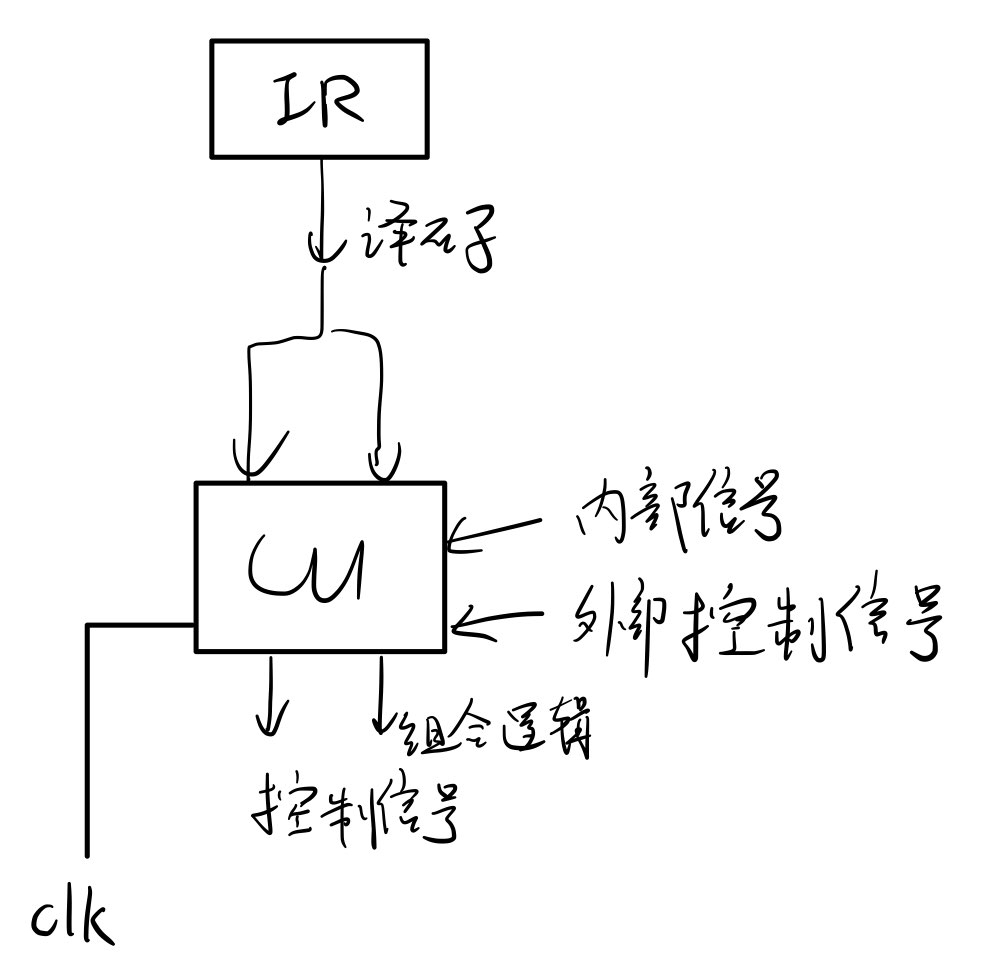
\includegraphics[width=5.5cm]{fig/10.7.png}
        \caption{10.7题图}
        \label{fig:10_7}
    \end{figure}

    指令处理过程分为四个阶段, 分别为取指周期, 间址周期, 执行周期和中断周期, 并且间址周期可能不使用, 中断周期也可能并不进入. 取指阶段的工作如下:

    \begin{enumerate}
        \item 经过CU输出的控制信号的控制, 从主存中取出指令, 存入指令寄存器IR中. 
        \item 从IR中取出指令, 经过指令译码器的译码与CU的逻辑电路, 产生相应的控制信号. 
        \item 控制信号送到控制单元 (比如控制某线路/总线上的信号是否可通), 控制单元根据控制信号控制各部件的工作.
    \end{enumerate}

    间址阶段的工作如下:

    \begin{enumerate}
        \item 从IR中取出指令 (中的一部分, 用来作为间址地址), 经过指令译码器的译码与CU的逻辑电路, 产生相应的控制信号. 
        \item 控制信号送到控制单元 (比如控制某线路/总线上的信号是否可通), 控制单元根据控制信号控制各部件的工作, 在这里是访存获得数据, 然后存入相应的寄存器 (比如覆写IR的地址部分).
    \end{enumerate}

    执行阶段的工作为: 根据指令在CU中产生的信号, 控制线路进行数据传输, 比如从寄存器中取出数据, 存入寄存器中, 或者从寄存器中取出数据, 送到ALU中进行运算, 然后将结果存入寄存器中, 也可能是和内存进行数据传输.

    中断阶段的工作为: 根据中断信号决定是否进入中断周期, 若进入, 则从PC中取出下一条指令的地址, 存入相应的寄存器中, 然后跳转到中断处理程序中.
\end{solution}


\problem{10.8} 画出微程序控制单元的组成框图, 根据指令处理过程, 结合有关部件说明其工作原理. 

\begin{solution}
    如图\ref{fig:10_8}所示. 这里是简化之后的版本, 省略了CMAR这个寄存器.
    \begin{figure}[!htbp]
        \centering
        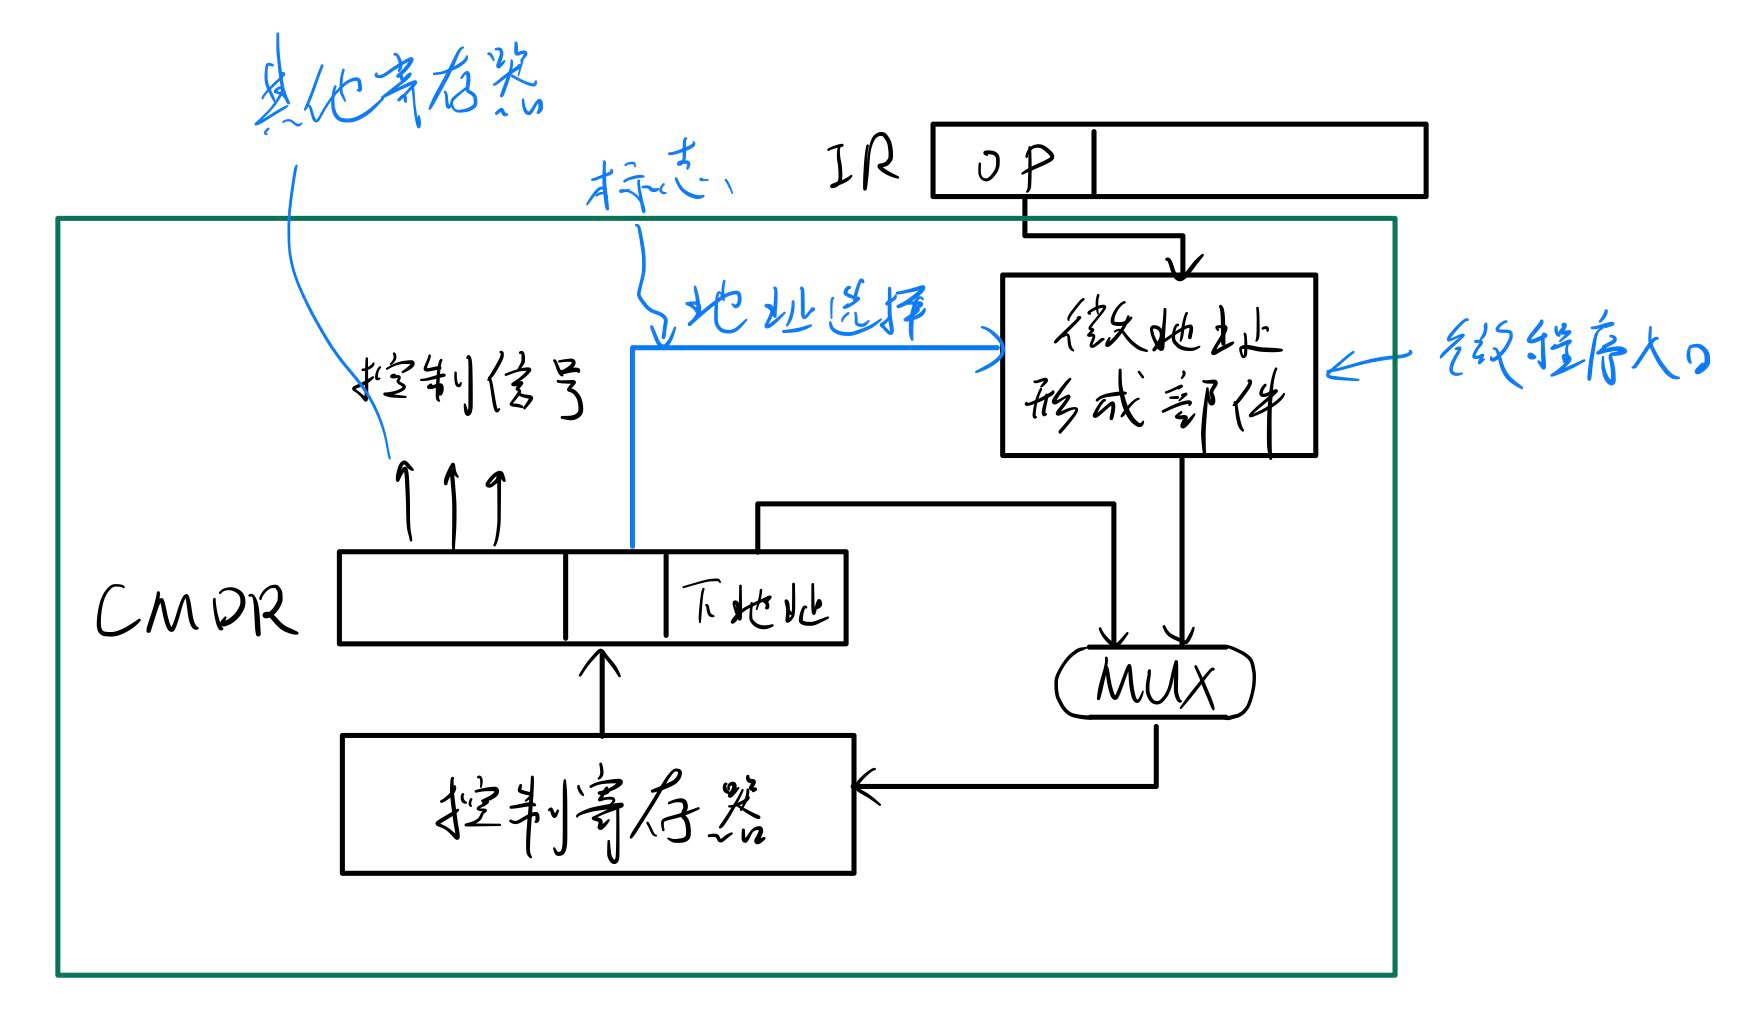
\includegraphics[width=9cm]{fig/10.8.png}
        \caption{10.8题图}
        \label{fig:10_8}
    \end{figure}

    指令处理过程分为四个阶段, 分别为取指周期, 间址周期, 执行周期和中断周期, 并且间址周期可能不使用, 中断周期也可能并不进入. 取指阶段的工作如下:

    \begin{enumerate}
        \item 读取微指令存储器中的微指令, 存入控制寄存器中, 然后微指令寄存器中取出微指令发送到CMDR.
        \item 微指令解码后, 发送控制信号给逻辑电路, 产生相应的控制信号. 控制信号送到控制单元外 (比如控制某线路/总线上的信号是否可通), 各部件根据控制信号工作, 实现取出PC送到IR的操作.
        \item 以上和以下操作, 都是依靠重复地选择进入下一条微指令的地址, 存入微指令地址寄存器中, 然后执行微指令来实现的.
    \end{enumerate}

    间址阶段的工作如下: 取微指令, 根据微程序中得到的控制信号, 从IR中取出指令 (中的一部分, 用来作为间址地址), 经过访存获得数据, 然后覆写IR的地址部分.

    执行阶段和中断阶段的工作和上面的基本相同.
\end{solution}


\problem{10.15} 设控制存储器的容量为$512 \times 48$位, 微程序可在整个控存空间实现转移, 而控制微程序转移的条件共有$4$个 (采用直接控制) , 微指令格式如图\ref{fig:10_15}. 试问微指令中的$3$个字段分别为多少位?
\begin{figure}[!htbp]
    \centering
    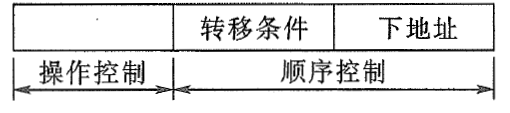
\includegraphics[width=5cm]{fig/10.15.png}
    \caption{10.15题图}
    \label{fig:10_15}
\end{figure}

\begin{solution}
    按照水平型 (水平微程序) 的微指令格式, 由于控制存储器的容量为$512 \times 48$位, 下地址需要$9$位来存储 ($2^9=512$); 由于转移的条件共有$4$个, 因此转移条件需要$4$位 (每一位代表一个转移条件); 剩余的$35$位均可留给操作控制段.
\end{solution}


\problem{10.21} 表\ref{tab:10_21_1}给出$8$条微指令$\mathrm{I_1}$~$\mathrm{I_8}$及所包含的微命令控制信号, 设计微指令操作控制字段格式, 要求所使用的控制位最少, 而且保持微指令本身内在的并行性. 
\begin{table}[htbp]
    \centering
    \caption{题10.21表}
    \begin{tabular}{l|l}
        \hline
        微指令 & 所含的微指令 \bigstrut\\
        \hline
        $\mathrm{I_1}$ & a b c d e \bigstrut\\
        \hline
        $\mathrm{I_2}$ & a d f g \bigstrut\\
        \hline
        $\mathrm{I_3}$ & b h \bigstrut\\
        \hline
        $\mathrm{I_4}$ & c \bigstrut\\
        \hline
        $\mathrm{I_5}$ & c e g i \bigstrut\\
        \hline
        $\mathrm{I_6}$ & a h j \bigstrut\\
        \hline
        $\mathrm{I_7}$ & c d h \bigstrut\\
        \hline
        $\mathrm{I_8}$ & a b h \bigstrut\\
        \hline
    \end{tabular}%
    \label{tab:10_21_1}%
\end{table}%

\begin{solution}
    先将微指令与对应的微命令绘制成表格, 并挖掘微命令的并行性, 将之重叠, 如表\ref{tab:10_21_2}所示.
    \begin{table}[htbp]
        \centering
        \caption{微操作与微命令并行对应}
        \begin{tabular}{|c|c|c|c|c|c|c|c|c|c|c|}
        \hline
        \multirow{2}[4]{*}{微操作码} & \multicolumn{10}{c|}{所含的微指令} \bigstrut\\
    \cline{2-11}      & \cellcolor[rgb]{ .867,  .851,  .769}\textbf{a} & \cellcolor[rgb]{ .867,  .851,  .769}\textbf{bgj} & \cellcolor[rgb]{ .867,  .851,  .769}\textbf{c} & \cellcolor[rgb]{ .867,  .851,  .769}\textbf{d} & \cellcolor[rgb]{ .867,  .851,  .769}\textbf{e} & \cellcolor[rgb]{ .867,  .851,  .769}\textbf{fhi} & g & h & i & j \bigstrut\\
        \hline
        $I_1$ & \cellcolor[rgb]{ 1,  1,  0}1 & \cellcolor[rgb]{ 1,  1,  0}1 & \cellcolor[rgb]{ 1,  1,  0}1 & \cellcolor[rgb]{ 1,  1,  0}1 & \cellcolor[rgb]{ 1,  1,  0}1 &   &   &   &   &  \bigstrut\\
        \hline
        $I_2$ & \cellcolor[rgb]{ 1,  1,  0}1 & \cellcolor[rgb]{ .922,  .945,  .871}1 &   & \cellcolor[rgb]{ 1,  1,  0}1 &   & \cellcolor[rgb]{ 1,  1,  0}1 & \cellcolor[rgb]{ .922,  .945,  .871}1 &   &   &  \bigstrut\\
        \hline
        $I_3$ &   & \cellcolor[rgb]{ 1,  1,  0}1 &   &   &   & \cellcolor[rgb]{ .722,  .8,  .894}1 &   & \cellcolor[rgb]{ .722,  .8,  .894}1 &   &  \bigstrut\\
        \hline
        $I_4$ &   &   & \cellcolor[rgb]{ 1,  1,  0}1 &   &   &   &   &   &   &  \bigstrut\\
        \hline
        $I_5$ &   & \cellcolor[rgb]{ .922,  .945,  .871}1 & \cellcolor[rgb]{ 1,  1,  0}1 &   & \cellcolor[rgb]{ 1,  1,  0}1 & \cellcolor[rgb]{ .992,  .914,  .851}1 & \cellcolor[rgb]{ .922,  .945,  .871}1 &   & \cellcolor[rgb]{ .992,  .914,  .851}1 &  \bigstrut\\
        \hline
        $I_6$ & \cellcolor[rgb]{ 1,  1,  0}1 & \cellcolor[rgb]{ .949,  .863,  .859}1 &   &   &   & \cellcolor[rgb]{ .722,  .8,  .894}1 &   & \cellcolor[rgb]{ .722,  .8,  .894}1 &   & \cellcolor[rgb]{ .949,  .863,  .859}1 \bigstrut\\
        \hline
        $I_7$ &   &   & \cellcolor[rgb]{ 1,  1,  0}1 & \cellcolor[rgb]{ 1,  1,  0}1 &   & \cellcolor[rgb]{ .722,  .8,  .894}1 &   & \cellcolor[rgb]{ .722,  .8,  .894}1 &   &  \bigstrut\\
        \hline
        $I_8$ & \cellcolor[rgb]{ 1,  1,  0}1 & \cellcolor[rgb]{ 1,  1,  0}1 &   &   &   & \cellcolor[rgb]{ .722,  .8,  .894}1 &   & \cellcolor[rgb]{ .722,  .8,  .894}1 &   &  \bigstrut\\
        \hline
        \end{tabular}%
        \label{tab:10_21_2}%
    \end{table}%

    \newpage
    
    这样, 我们可以用$1 \cdot 4 + 2 \cdot 2 = 8$位作为控制位, 分别对应 a bgj c d e fhi. 这六段的表示如表\ref{tab:10_21_3}所示.
    \begin{table}[htbp]
        \centering
        \caption{微操作控制位与微命令的对应}
        \begin{tabular}{|c|c|c|c|c|}
            \hline
            \textbf{编码} & \textbf{0} & \textbf{1} & \textbf{2} & \textbf{3} \bigstrut\\
            \hline
            \rowcolor[rgb]{ .867,  .851,  .769} \textbf{a} & \cellcolor[rgb]{ 1,  1,  1}无操作 & \cellcolor[rgb]{ 1,  1,  1}微命令a & \multicolumn{2}{c|}{\cellcolor[rgb]{ 1,  1,  1}} \bigstrut\\
            \hline
            \rowcolor[rgb]{ .867,  .851,  .769} \textbf{bgj} & \cellcolor[rgb]{ 1,  1,  1}无操作 & \cellcolor[rgb]{ 1,  1,  1}微命令b & \cellcolor[rgb]{ 1,  1,  1}微命令g & \cellcolor[rgb]{ 1,  1,  1}微命令j \bigstrut\\
            \hline
            \rowcolor[rgb]{ .867,  .851,  .769} \textbf{c} & \cellcolor[rgb]{ 1,  1,  1}无操作 & \cellcolor[rgb]{ 1,  1,  1}微命令c & \multicolumn{2}{c|}{\cellcolor[rgb]{ 1,  1,  1}} \bigstrut\\
            \hline
            \rowcolor[rgb]{ .867,  .851,  .769} \textbf{d} & \cellcolor[rgb]{ 1,  1,  1}无操作 & \cellcolor[rgb]{ 1,  1,  1}微命令d & \multicolumn{2}{c|}{\cellcolor[rgb]{ 1,  1,  1}} \bigstrut\\
            \hline
            \rowcolor[rgb]{ .867,  .851,  .769} \textbf{e} & \cellcolor[rgb]{ 1,  1,  1}无操作 & \cellcolor[rgb]{ 1,  1,  1}微命令e & \multicolumn{2}{c|}{\cellcolor[rgb]{ 1,  1,  1}} \bigstrut\\
            \hline
            \rowcolor[rgb]{ .867,  .851,  .769} \textbf{fhi} & \cellcolor[rgb]{ 1,  1,  1}无操作 & \cellcolor[rgb]{ 1,  1,  1}微命令f & \cellcolor[rgb]{ 1,  1,  1}微命令h & \cellcolor[rgb]{ 1,  1,  1}微命令i \bigstrut\\
            \hline
        \end{tabular}%
        \label{tab:10_21_3}%
    \end{table}%

    如果用直接控制阀需要10位, 而这里只需要8位, 因此可以减少2位.
\end{solution}









\end{document}